\newpage
\section{Auswertung}
    \subsection{Bestimmung des Kernspins}
        Um den Kernspin bestimmen zu können nutzt man den linearen Zusammenhang zwischen der Energie der Zeemann-Aufspaltung und des angelegten horizontalen B-Feldes. Da die Energie der Zeemann-Aufspaltung 
        in diesem Versuch proportional zur Frequenz des RF-Feldes ist, wird das angelegte B-Feld gegen diese aufgetragen. Dazu müssen zunächst über das Helmholtz-Gesetz (Referenz) aus den Spulenspannungen 
        \ref{tab:daten} die zugehörigen B-Felder für die Horizontale- und Sweep-Spule berechnet und anschließend addiert werden (\ref{tab:daten}).  
        
        
        \FloatBarrier

        \begin{figure}[h]
          \centering
          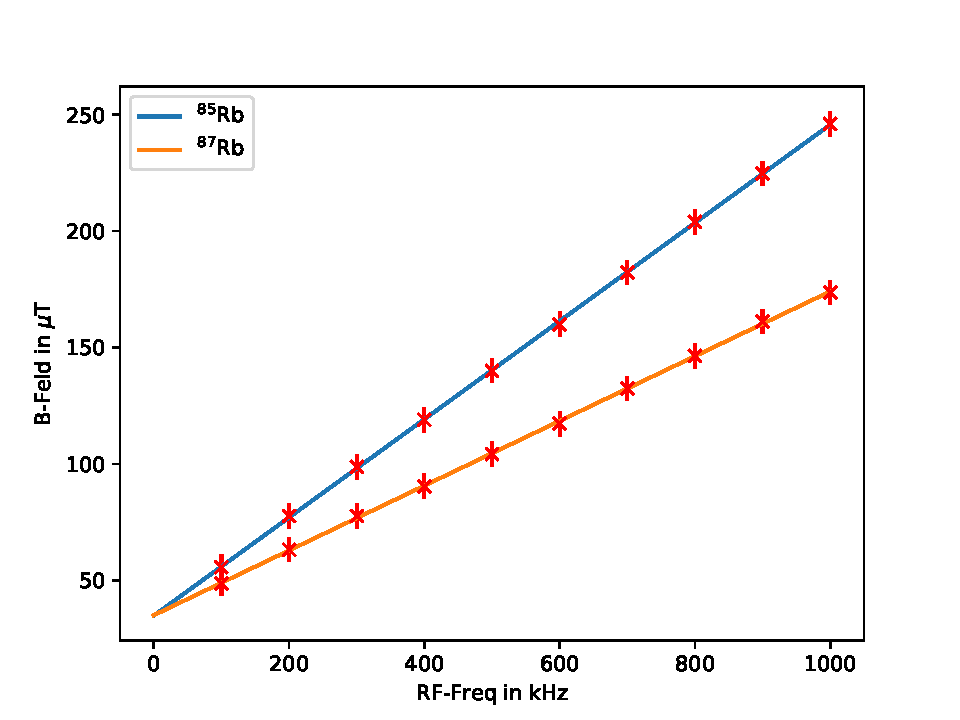
\includegraphics[width = 0.6\textwidth]{pictures/Rb_85_87.pdf}
          \caption{In der Abbildung sind die angelgten horizontalen Magnetfeldstärken gegen die zugehörigen RF-Frequenzen aufgetragen. }
          \label{fig:B_gegen_RF}
        \end{figure}

        \FloatBarrier

        \noindent
        
        
        
        Da zwei Rubidium-Isotope vorhanden sind, werden auch zwei Geraden geplotted. Der Lande-Faktor, aus dem der Kernspin bestimmt werden soll, ist der Teil der Steigung der aufgetragenen Geraden. Daher 
        werden für beide Isotope lineare Ausgleichsgeraden gefitted und aus der zugehörigen Steigung m die Lande-Faktoren bestimmt:

        \begin{align*}
            \text{B}(f) &= \text{m} \cdot f &+ \text{b}   \\
            \text{B}(f) &= \frac{4 \pi \text{m}_{\text{e}}}{\text{e} \text{g}_{\text{F}}} \cdot f &+ \text{B}_0 
        \end{align*}

        \begin{align*}
            \text{${}^{85}$Rb} &: \, \text{m} = \num{2107.3\pm6.9 e-13} \, \longrightarrow \, \text{g}_{\text{F, ${}^{85}$Rb}} = \num{0.3390 +- 0.0011} \\
            \text{${}^{87}$Rb} &: \, \text{m} = \num{1389.8\pm7.8 e-13} \, \longrightarrow \, \text{g}_{\text{F, ${}^{87}$Rb}} = \num{0.5141 +- 0.0029} 
        \end{align*}

        \noindent

        Um aus diesen Lande-Faktoren den Kernspin zu bestimmen, wird der Zusammenhang zwischen $\text{g}_{\text{F}}$ und $\text{g}_{\text{J}}$, in dem auch der Kernspin I enthalten ist (Referenz), nach 
        eben diesem umgestellt:
        
        \begin{equation*}
            \text{I} = \left( \frac{\text{g}_{\text{J}}}{\text{g}_{\text{F}}} - 1 \right) \cdot \text{J}
        \end{equation*}

        $\text{g}_{\text{J}}$ berechnet sich für Rubidium nach (Referenz) zu 2 und J ist mit $\frac{1}{2}$ gegeben, sodass sich folgende Kernspins berechnen lassen:

        \begin{equation*}
            \text{I}_{\text{${}^{85}$Rb}} = \num{2.449 +- 0.010} \qquad \text{I}_{\text{${}^{87}$Rb}} = \num{1.445 +- 0.011}
        \end{equation*}

        

    \subsection{Abschätzung des quadratischen Zeemann-Effekts}
        Da der quadratische Zeemann-Effekt bei höheren Magnetfeldstärken auftritt, wird die Größe der zugehörigen Energieaufspaltung für die maximal angelegten Magnetfeldstärken berechnet. So ergeben sich mit 
        den angebeben Hyperfeinstrukturaufspaltungen $\Delta\text{E}_{\text{HFS}, {}^{85}\text{Rb}} =  \SI{2.01 e-24}{\joule}$, $\Delta\text{E}_{\text{HFS}, {}^{87}\text{Rb}} = \SI{4.53 e-24}{\joule}$ und 
        maximalen Magnetfeldstärken folgende Energieaufspaltungen:

        \begin{align*}
            \Delta\text{E}_{\text{QZ}, {}^{85}\text{Rb}} (\SI{246 +- 5}{\micro\tesla})= \SI{2.89\pm0.13 e-31}{\joule} \\
            \Delta\text{E}_{\text{QZ}, {}^{87}\text{Rb}} (\SI{174 +- 5}{\micro\tesla})= \SI{1.51\pm0.09 e-31}{\joule}
        \end{align*}



    \subsection{Bestimmung des Isotopenverhältnisses}
        Das Verhältnis zwischen den beiden Rubidium-Isotopen in der Dampfzelle kann direkt aus den Dips des Oszilloskopbildes abgelesen werde. Das Verhätlnis derer Stärke entspricht auch dem Mengenverhältnis
        der beiden Isotope.


        \FloatBarrier

        \begin{figure}[h]
          \centering
          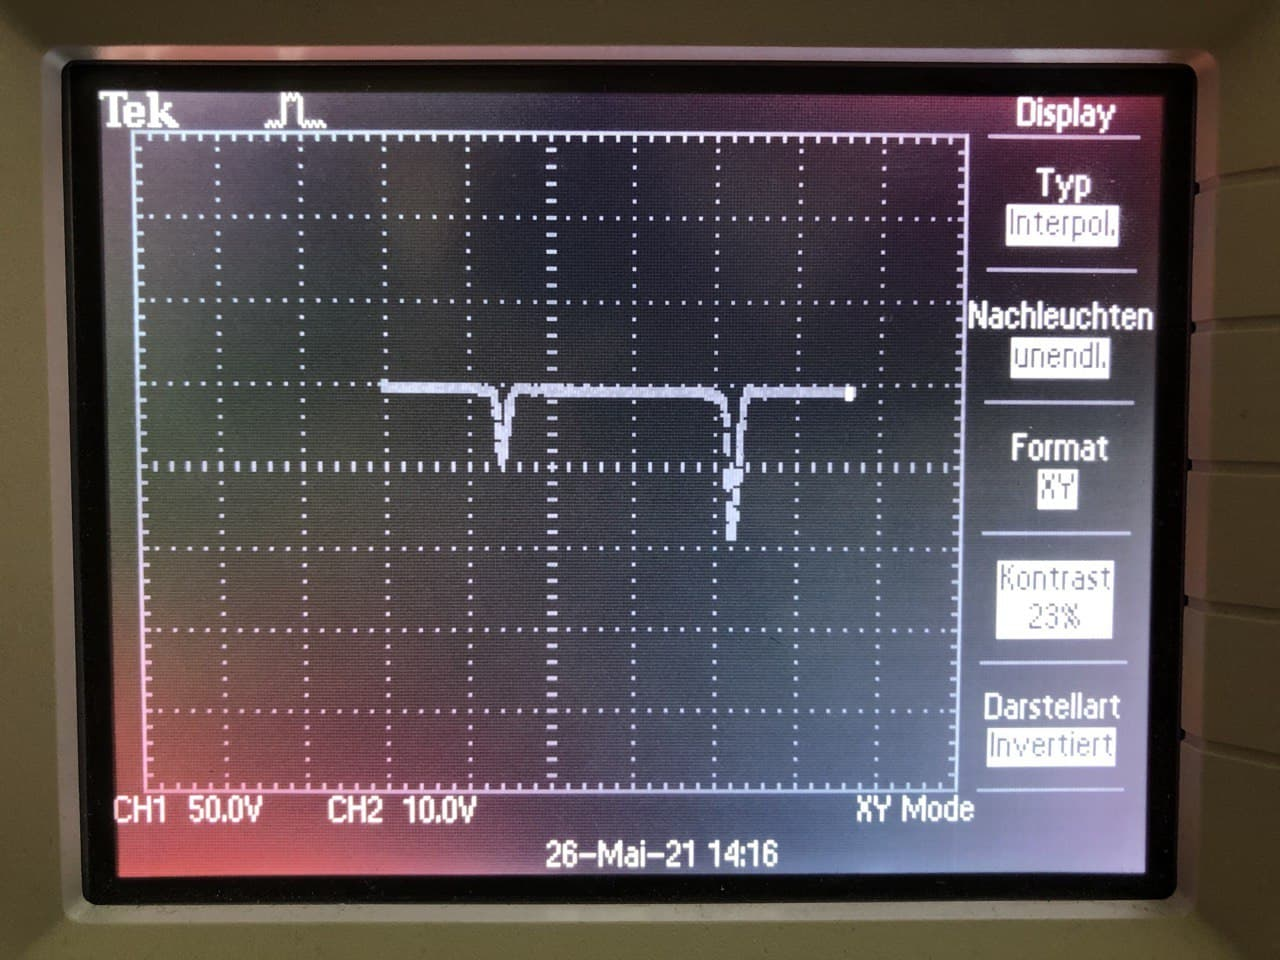
\includegraphics[width = 0.6\textwidth]{pictures/isotop_vergleich.jpg}
          \caption{In der Abbildung sind die Einbrüche der Transmission zu sehen. Der erste Einbruch gehört zu ${}^{87}$Rb und der zweite zu ${}^{85}$Rb.}
          \label{fig:isotop_vergleich}
        \end{figure}

        \FloatBarrier

        \noindent

        Aus Abbildung \autoref{fig:isotop_vergleich} ist zu erkennen, dass ${}^{85}$Rb in etwa doppelt so oft vorkommt wie ${}^{87}$Rb.



        \subsection{Bestimmung des Erdmagnetfeldes}

        Zur Bestimmung der horizontalen Komponente des Erdmagnetfeldes wird wieder die Ausgleichsgerade aus Grafik \autoref{fig:B_gegen_RF} verwendet. Die jeweiligen y-Achsen-Abschnitte geben direkt die 
        horizontale Magnetfeldstärke, sodass nur zwischen den beiden Werten gemittel werden muss.
        
        \begin{equation*}
            \text{b}_{\text{${}^{85}$Rb}}= \num{349.4\pm4.3 e-7} \qquad \text{b}_{\text{${}^{85}$Rb}}= \num{351.1\pm4.9 e-7} \qquad \longrightarrow \qquad  \overline{\text{B}_{\text{hor}}} = \SI{35.02 +- 0.32}{\micro\tesla}
        \end{equation*}
    
        \noindent

        Die vertikale Komponente kann unter der Annahme, dass diese durch die vertikale Spule zu Beginn genau kompensiert wurde, direkt aus dem Magnetfeld der vertikalen Spule berechnet werden. Mit dem 
        Helmholtz-Gesetz ergibt sich so folgende vertikale Magnetfeldstärke:

        \begin{equation*}
            \text{B}_{\text{vert}} = \SI{34.63 +- 0.15}{\micro\tesla}
        \end{equation*}

